\documentclass[lang=cn,11pt]{template}

\usepackage{amsmath}%
\usepackage{amssymb}%
\usepackage{pdfpages}
\title{395 Homework}
\author{Qiulin Fan}
\begin{document}   
\frontmatter
\tableofcontents
\mainmatter



\chapter{on metric spaces}

\section{rooted metric gives $(0,1)$ infinite length}
Suppose \((X, d)\) is a metric space. For \(0 < \epsilon < 1\), show that \(d^\epsilon\) is also a metric on \(X\).

If \(X = [0, 1]\) is the unit interval and \(d\) is the usual metric, show that \(X\) has "infinite length" using the metric \(d^\epsilon\), in that

\[
\sup_{0 = t_0 < t_1 < \cdots < t_n = 1} \sum_{i=1}^{n} d^\epsilon(t_i, t_{i-1}) = \infty.
\]

Here the supremum is taken over all \(n\) and all \(n + 1\) tuples of points \(t_i\) as in the subscript.

\textit{Optional context:} If you’d like to know where the metrics \(d^\epsilon\) appear, try looking up the Assouad Embedding Theorem. If you’d like to know more about the notion of length used here, try looking up rectifiable curves.



\section{Matrix chain multiplication}
If \(X\) is an \(a \times b\) matrix, and \(Y\) is a \(b \times c\) matrix, it takes \(abc\) multiplications to compute \(XY\) according to the usual formula for matrix multiplication. (There are \(ac\) entries in \(XY\), and each is a sum of \(b\) products.) Thus, let’s estimate the time it takes to multiply these two matrices as \(abc\).

Say \(A_1\) is a \(5 \times 1\) matrix, \(A_2\) is a \(1 \times 5\) matrix, \(A_3\) is a \(5 \times 2\) matrix, \(A_4\) is a \(2 \times 5\) matrix, \(A_5\) is a \(5 \times 1\) matrix, and \(A_6\) is a \(1 \times 10\) matrix.

If you want to compute \(A_1 A_2 A_3 A_4 A_5 A_6\), how should you bracket this product so that the sum of the time estimates for the multiplications is as small as possible? For example, should you do
\[
(A_1 (A_2 A_3)) ((A_4 A_5) A_6)?
\]
Or
\[
(A_1 (A_2 (A_3 (A_4 (A_5 A_6)))))?
\]
Or something else?
HintL: Wikipedia entry titled “Matrix chain multiplication.”
\begin{solution}
    Dynamic Programming. I have no idea why it appears here, but it is dynamic programming.
\end{solution}

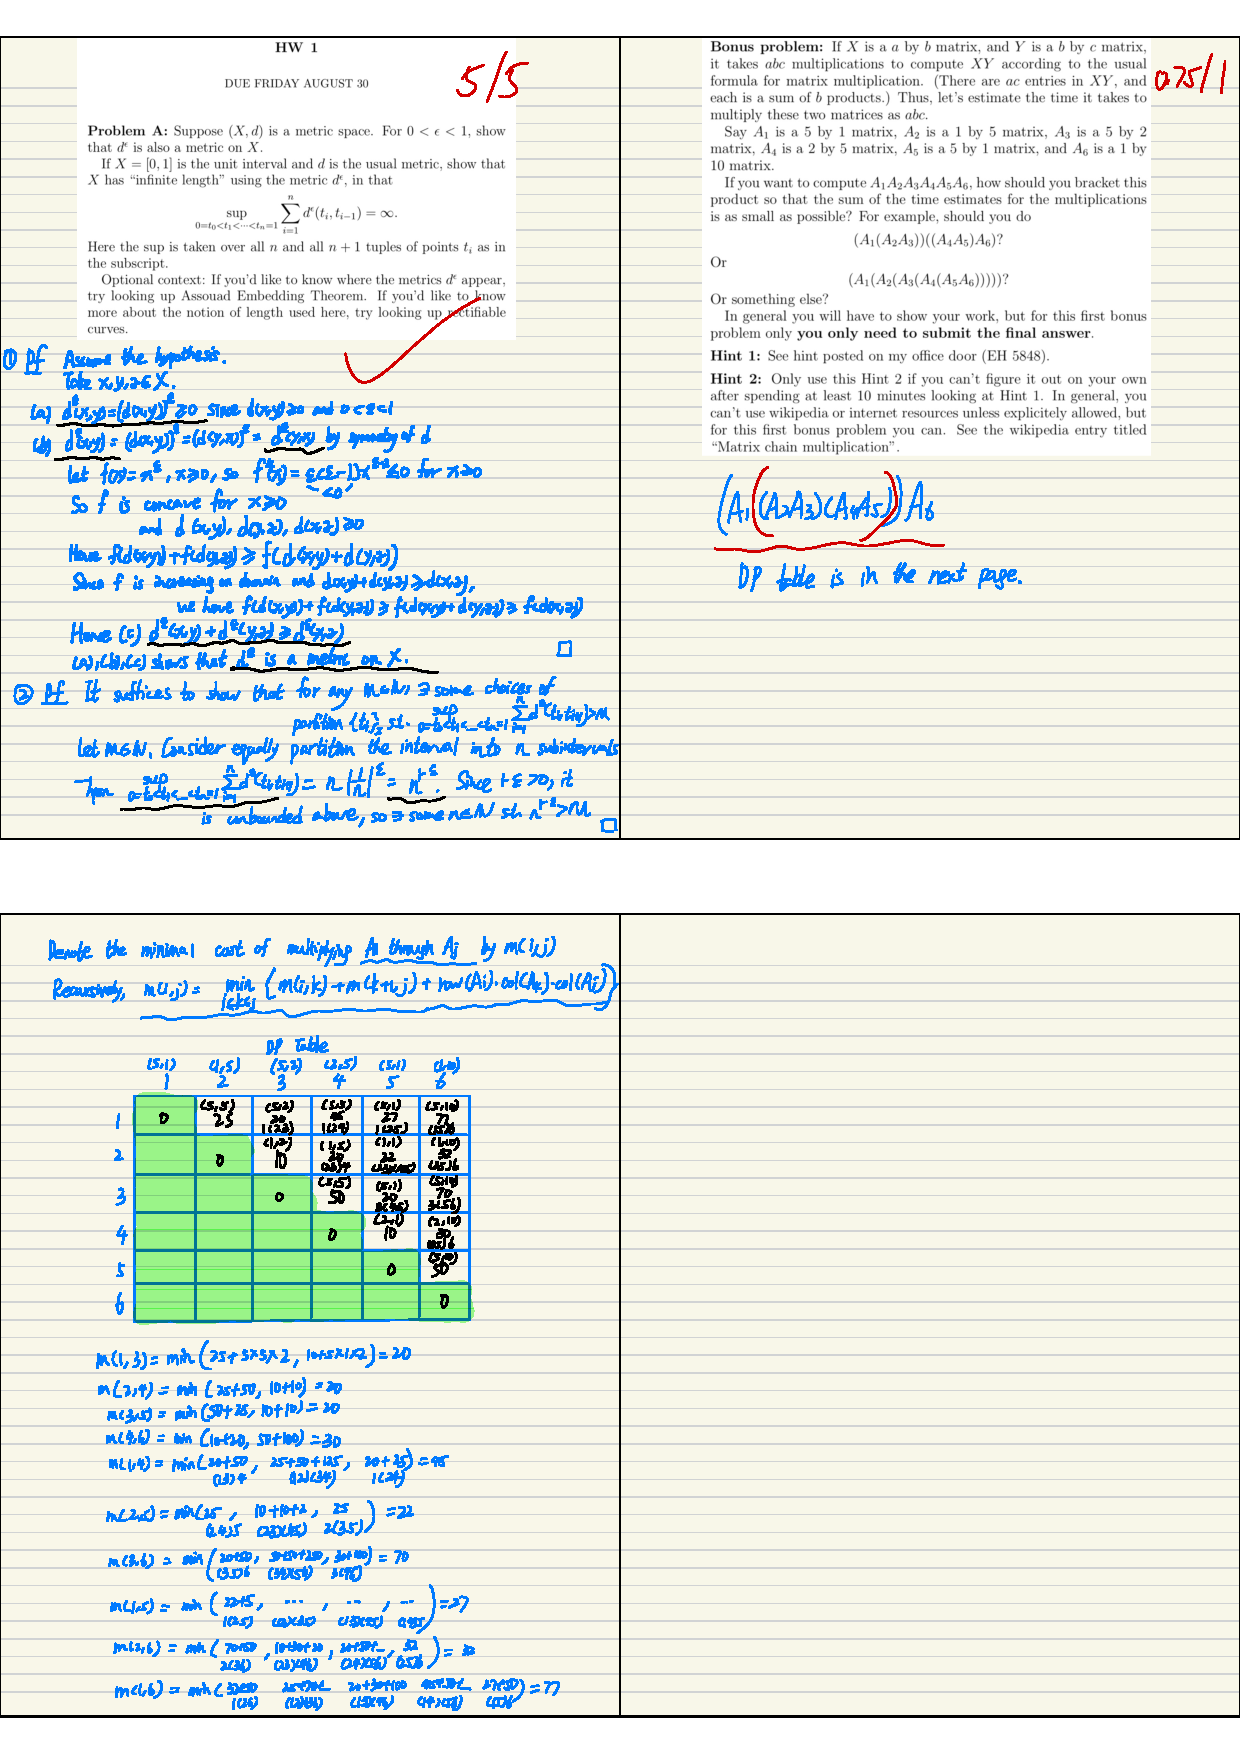
\includepdf[pages=-]{395-hw-01.pdf}



\chapter{on ttl bdd, sup norm and cptness}

\section{metric induced by vector norm}
\begin{definition}
    \textbf{normed vector space:} 
    \\vector space 上可以定义 norm 来表示每个 vector 的“大小”,norm 的定义是满足\\ \textbf{(1) positive definiteness; (2) homogeneity (3) triangle ineq 的 $||.||: V \rightarrow \mathbb{R}_{\geq0}$}
\end{definition}
If \( \|\cdot\| \) is a norm on a vector space \( V \), show that \( d(x, y) = \|x - y\| \) defines a metric on \( V \).

\section{operator norm: linear map is ctn iff bdd (因而有限维 vector spaces 间的 linear operator 一定 ctn 且 bdd)}

\begin{definition}{operator norm}\label{operator norm}
Let \( T: V_1 \to V_2 \) be a linear map between normed vector spaces. The norm on \( V_i \) will be denoted \( \|\cdot\|_i \). Define

\[
\|T\| = \sup_{v \in V_1, v \neq 0} \frac{\|T v\|_2}{\|v\|_1} = \sup_{v \in V_1, \|v\|_1 = 1} \|T v\|_2.
\]

This is either a non-negative real number or infinity. The linear map is called bounded if it is not infinity. Show that \( T \) is continuous if and only if it is bounded.

\end{definition}

\begin{remark}
    给定两个 normed vector spaces $V_1, V_2$,我们实际上也 induce 出了 $Hom(V_1, V_2)$ 上的一个 norm, 即此处的 operator norm.\\
    $Hom(V_1, V_2)$ 上还可以定义 Frobenious norm (treat like $\bR^{n \times n}$) 以及 sup norm (sup norm in $\bR^{n \times n}$).
\end{remark}

\begin{remark}
  我们可以用 $||T(v) - T(w)||_2 \rightarrow 0$ as $||v - w||_1 \rightarrow 0$ (或者 sequentially)来定义 \textbf{continuous by norm}.  
\end{remark}

\begin{theorem}{Finite dim VS 上 linear map bdd 且 ctn}\label{Finite dim VS 上 linear map bdd 且 ctn}
    (1) \textbf{linear map bounded 当且仅当它 continuous.}
    (2)  \textbf{有限维度的 vector space 之间的任意 linear map 一定 bounded(}因为一定可以选择 base 然后把线性变换用 matrix 来表示),所以一定 continuous.
\end{theorem}




\section{unbounded linear map in infinite dim vector space}
\begin{enumerate}
    \item Give an example of an unbounded linear map.
    \begin{solution}
        一个 infinite dimension 的 vector space 的 unbounded linear map 的例子: $$T = \frac{d}{dx}|_{x=0} \in Hom(C[0,1], \mathbb{R})$$
    \end{solution}
    \item Give an example of a sequence \( (T_i) \) of diagonalizable \( 2 \times 2 \) real matrices whose eigenvalues stay bounded but for which \( \|T_i\| \to \infty \). (Here the matrices define linear maps from \( \mathbb{R}^2 \) to itself, and we use the Euclidean norm on \( \mathbb{R}^2 \).)
\end{enumerate}

\section{ttl bdd metric space 一定 separable (有 ctbl dense subset)}
Show that if a subset of a metric space is totally bounded, then it is also separable (i.e., there exists a countable dense subset).

\begin{remark}
    如果一个 metric space $X$ 是 separable 的,那么随意 enumerate 一个 dense sequence $(p_n)$,这个 sequence 的所有 subsequential limit 就是整个 $X$. 即对于 $X$ 中任意一个元素,都可以找到 $(p_n)$ 的一个 subsequence 使得它的 limit 是整个元素
\end{remark}


\section{quotient topology}
Let \( X \) be defined as infinitely many copies of \( [0, 1] \) with all their left endpoints glued together, with the natural metric \( d \).

Formally, we can first define \( \hat{X} = \mathbb{N} \times [0, 1] \), and define an equivalence relation on \( \hat{X} \) by \( (i, x) \sim (j, y) \) if and only if \( (i, x) = (j, y) \) or \( x = y = 0 \). Let \( X \) be the set of equivalence classes, and define a metric \( d \) by setting

\[
d([ (i, x) ], [ (j, y) ]) = |x| + |y| \quad \text{if } i \neq j \quad \text{and} \quad d([ (i, x) ], [ (j, y) ]) = |x - y| \quad \text{if } i = j.
\]

You should convince yourself that this makes sense but don’t have to write this up.

Prove that \( (X, d) \) is bounded but not totally bounded.

\section{space of converging sequence 中 ttl bdd 的判断标准}
Let \( c_0 \) be the subspace of \( \ell^\infty(\mathbb{N}) \) of sequences that converge to zero, with the sup metric. Show that a subset \( Q \) of \( c_0 \) is totally bounded if and only if it is bounded and for all \( \epsilon > 0 \), there exists \( N > 0 \) such that for all \( (x_n) \in Q \) and all \( n \geq N \), we have \( |x_n| < \epsilon \).


\begin{remark}
$l^{\infty}(\mathbb{N})$ 中的所有收敛到 0 的序列构成的集合,称之为 $l_0^{\infty}(\mathbb{N})$,这个集合 \textbf{$l_0^{\infty}(\mathbb{N})$ 从 bdd 提升到 ttl bdd 所需要的条件是其中所有序列是uniformly收敛的.}
    
\end{remark}


\section{Bonus: isometry embedding}
A map \( f: X \to Y \) between metric spaces is called an isometric embedding if

\[
d(f(x_1), f(x_2)) = d(x_1, x_2)
\]

for all \( x_1, x_2 \in X \). If such a map exists, we say \( X \) embeds isometrically in \( Y \).

Show that every separable metric space embeds isometrically into \( \ell^\infty(\mathbb{N}) \).

\begin{definition}
    \textbf{isometric embedding}: \\
    如果两个 metric space 之间的一个 map\textbf{ 保留 distance (即 $\forall x,y \in X, $ $d(f(x), f(y)) = d(x,y)$)} 那么就称这个 map 为一个 isometric embedding.
\end{definition}

\begin{theorem}
    \textbf{任意 separable metric space 都可以 embedds isometrically into $l^{\infty}(\mathbb{N})$.}
\end{theorem}

\proof 构造:首先 enumeate  $X$ 的一个 dense sequence $(p_n)$,并取它的首项 $p_1$,然后对于每个 $x \in X$, induce 出 $(d_X(x, p_n) - d_X(p_0, p_n))_{n \in \mathbb{N}}$ 这个序列. 可以发现从 $f: x \mapsto (d_X(x, p_n) - d_X(p_0, p_n))_{n \in \mathbb{N}}$ 是一个 isometry embedding. 

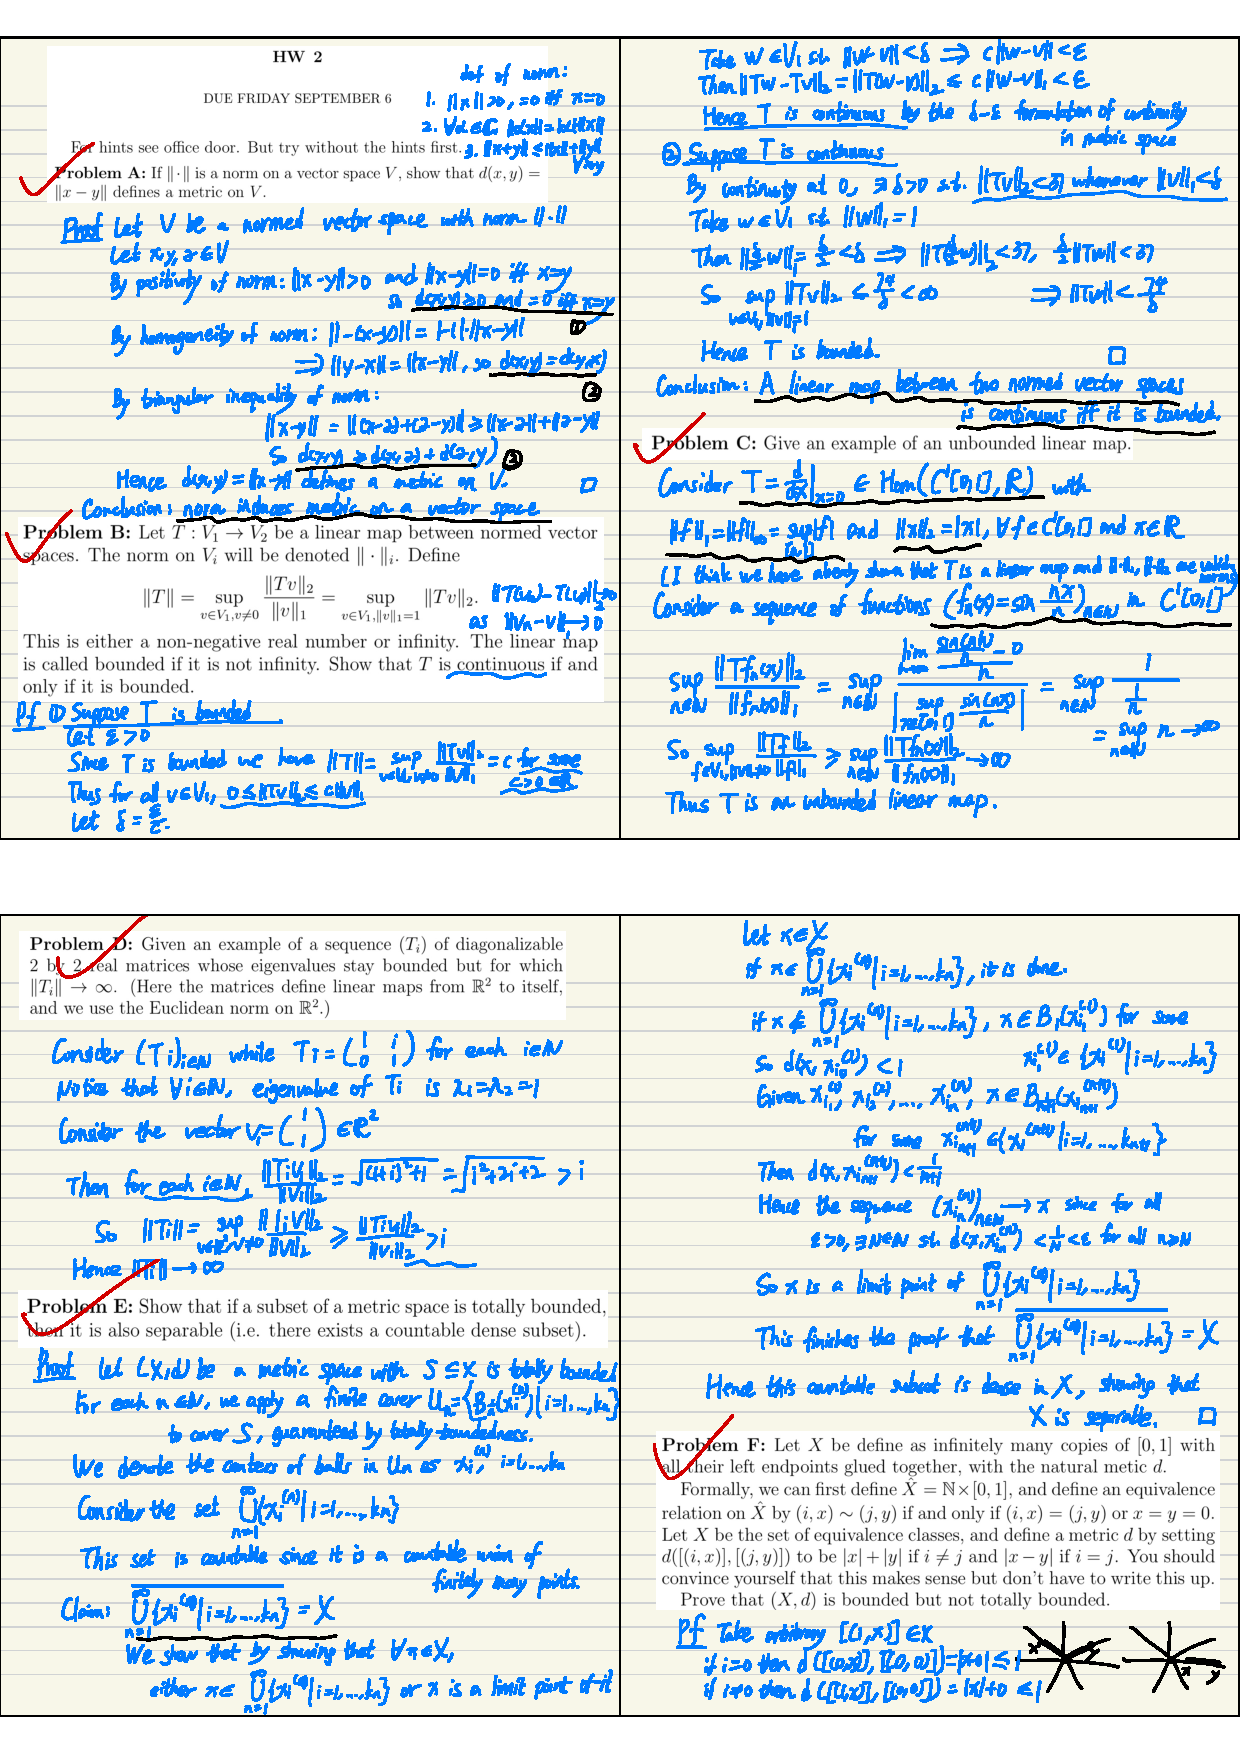
\includepdf[pages=-]{395-hw-02.pdf}




\chapter{on Lipschitz map and differentiation}
\section{Lipschitz condition: stronger than uniformly ctn}
Let \( (X_1, d_1) \) and \( (X_2, d_2) \) be two metric spaces. We say that a function \( f : X \to Y \) is Lipschitz with constant \( C \) if for any \( x, y \in X \), we have
\[
d_2(f(x), f(y)) \leq C d_1(x, y).
\]
\begin{enumerate}
    \item Show that Lipschitz maps are uniformly continuous, i.e., for all \( \epsilon > 0 \) there exists \( \delta > 0 \) such that if \( x_1, x_2 \in X \) and \( d_1(x_1, x_2) < \delta \), then \( d_2(f(x_1), f(x_2)) < \epsilon \).
    \item Let \( f_n : X_1 \to X_2 \) be Lipschitz maps with common Lipschitz constant \( C \). Suppose that \( f_n \) converges uniformly to \( f \), i.e., for all \( \epsilon > 0 \), there exists \( N > 0 \) such that for all \( n > N \) and all \( x \in X_1 \),
    \[
    d_2(f_n(x), f(x)) < \epsilon.
    \]
    Is \( f \) Lipschitz? What if we only assume that the \( f_n \) are Lipschitz (without giving a common Lipschitz constant)?
\end{enumerate}

\section{ctn map between topological spaces preserves connectness}
We say that a metric space \( X \) is connected if it cannot be written as \( X = A \cup B \) where \( A \) and \( B \) are nonempty disjoint open subsets of \( X \).
\begin{enumerate}
    \item Show that if \( f : X \to Y \) is a continuous function between metric spaces \( X \) and \( Y \), then \( f(X) \) is connected if \( X \) is connected.
    \item Conclude that if \( f : X \to \mathbb{R} \) and \( X \) is a connected metric space, then \( f \) admits all intermediate values \( m \in (\inf f, \sup f) \). That is, for any such \( m \), there exists \( x_0 \in X \) such that \( f(x_0) = m \).
\end{enumerate}

\section{ctn bijective map from a cpt topological space to a Hausdorff space is a homeomorphism}
Let \( f : X \to Y \) be a continuous bijective (one-to-one and onto) mapping between metric spaces \( X \) and \( Y \).
\begin{enumerate}
    \item Suppose that \( X \) is compact. Show that the inverse function \( f^{-1} : Y \to X \) is also continuous.
    \item Give an example to show that the requirement that \( X \) is compact is necessary.
\end{enumerate}
\begin{remark}
    实际上这个条件可更宽松. \textbf{任意一个 continuous bijective map from a compact topological space to a Hausdorff space 都是一个 homeomorphism.}\\
    这是因为 continuous function maps compact set to compact set, 而 \textbf{compact topological space 中的 closed set 一定 compact}; 且 \textbf{Hausdorff space 中 compact set 一定 closed.}\\ 
    所以任取 closed set in $X$, 由于 X compact, 这个集合也 compact; 且它的 preimage by $f^{-1}$ is closed since $f$ ctn. 因而 $f^{-1}$ 是 ctn 的.
\end{remark}


\section*{3D: an example of ctn but non-diffble point}
Let \( f \) be a real-valued function defined on \( \mathbb{R}^n \) (or an open subset of \( \mathbb{R}^n \)). Recall that the directional derivative \( D_v f(p) \) of \( f \) at \( p \) in the direction \( v \) is the vector
\[
D_v f(p) = \lim_{t \to 0} \frac{f(p + tv) - f(p)}{t}
\]
if this limit exists.
\begin{enumerate}
    \item If \( c \in \mathbb{R} \) and \( D_v f(p) \) exists, prove that \( D_{cv} f(p) \) exists and \( D_{cv} f(p) = c \cdot D_v f(p) \).
    \item For \( f : \mathbb{R}^2 \to \mathbb{R} \) defined by
    \[
    f(x, y) = \sqrt{|xy|}
    \]
    and \( v = (1, 0) \), \( v' = (0, 1) \), show that \( D_v f(0, 0) \) and \( D_{v'} f(0, 0) \) exist but \( D_{v+v'} f(0, 0) \) does not exist.
    \item Let \( f : \mathbb{R}^2 \to \mathbb{R} \) be defined by
    \[
    f(x, y) = \frac{xy^2}{x^2 + y^2}
    \]
    for \( (x, y) \neq (0, 0) \) and \( f(0, 0) = 0 \). Prove that \( D_v f(0, 0) \) exists for every \( v = (a, b) \in \mathbb{R}^2 \), vanishing if \( v = 0 \) and equal to
    \[
    \frac{ab^2}{a^2 + b^2}
    \]
    otherwise.
\end{enumerate}
Using polar coordinates, it is easy to see that \( f \) is continuous at \( (0, 0) \).

\begin{remark}
    如果 $f$ 在 $x$ 处 differentiable, 那么它的 $D_v(x)$ 是关于 $v$ linear 的; 如果在 $x$ 处 不 differentiable 则不然 (即便各个方向的偏导数都存在也不能保证.)
\end{remark}

\section{Bonus: uniformly disconnectness and ultrametric}
A metric space \( (X, d) \) is said to be uniformly disconnected if there is \( \epsilon_0 > 0 \) so that no pair of distinct points \( x, y \in X \) can be connected by an \( \epsilon_0 \)-chain, where an \( \epsilon_0 \)-chain connecting \( x \) and \( y \) is a sequence of points
\[
x = x_0, x_1, \dots, x_m = y
\]
satisfying
\[
d(x_i, x_{i+1}) \leq \epsilon_0 d(x, y).
\]
\begin{enumerate}
    \item Show that the Cantor set is uniformly disconnected.
    \item Show that a metric space \( (X, d) \) is uniformly disconnected if and only if there is an ultrametric \( d' \) on \( X \) for which there is some \( C > 1 \) such that
    \[
    \frac{d'(x, y)}{C} \leq d(x, y) \leq C d'(x, y).
    \]
\end{enumerate}
An ultrametric is a metric which satisfies the following improvement of the triangle inequality:
\[
d(x, z) \leq \max(d(x, y), d(y, z))
\]
for all \( x, y, z \). The discrete metric, where the distance between any pair of distinct points is 1, is an example of an ultrametric. Many other more interesting and important examples exist.

\includepdf[pages=-]{395-hw-03.pdf}




\chapter{on partial derivatives}

\section{在原点可导且保留 scalar 的函数一定是 linear map}
Let \( F : \mathbb{R}^n \to \mathbb{R}^m \) satisfy
\[
F(tx) = tF(x)
\]
for all positive real numbers \( t \) and all \( x \in \mathbb{R}^n \). Assume \( F \) is differentiable at the origin. Show that \( F \) is linear.

\section{all partials exist 且 bdd on $A$ $\implies$ ctn on $A$}
Let \( A \subset \mathbb{R}^n \) be open and \( f : A \to \mathbb{R}^m \). Suppose that the partial derivatives \( \frac{\partial f_i}{\partial x_j} \) (for \( 1 \leq i \leq m \) and \( 1 \leq j \leq n \)) exist and are bounded on \( A \). Show that \( f \) is continuous on \( A \).

\section{example of all partials exist and bounded 但不可导}
Let \( f : \mathbb{R}^2 \to \mathbb{R}^2 \) be defined by the equation:
\[
f(r, \theta) = (r \cos \theta, r \sin \theta).
\]
\begin{enumerate}
    \item Calculate \( Df \) and \( \det Df \).
    \item Let \( S = [1, 2] \times [0, \pi/2] \). Find \( f(S) \) and sketch it.
    \item Show that \( f \) is a homeomorphism from \( S \) onto \( f(S) \) and compute the inverse function \( f^{-1} \).
    \item Compute \( Df^{-1} \) and \( \det Df^{-1} \).
    \item What relation can you find between \( Df \) and \( Df^{-1} \)?
\end{enumerate}

\noindent\textbf{4D: }
Give an example of a function \( F : \mathbb{R}^2 \to \mathbb{R}^2 \) such that, at the origin, all directional derivatives exist and are zero, but \( F \) is not differentiable at the origin.\\

\noindent\textbf{4E: }
Define \( f : \mathbb{R}^2 \to \mathbb{R} \) by setting \( f(0) = 0 \) and
\[
f(x, y) = \frac{xy(x^2 - y^2)}{x^2 + y^2}.
\]
\begin{enumerate}
    \item Show that \( \frac{\partial f}{\partial x} \) and \( \frac{\partial f}{\partial y} \) exist at \( (0, 0) \).
    \item Compute \( \frac{\partial f}{\partial x} \) and \( \frac{\partial f}{\partial y} \) for \( (x, y) \neq 0 \).
    \item Show that \( f \in C^1(\mathbb{R}^2) \).
    \item Show that \( \frac{\partial}{\partial x} \left( \frac{\partial f}{\partial y} \right) \) and \( \frac{\partial}{\partial y} \left( \frac{\partial f}{\partial x} \right) \) exist everywhere on \( \mathbb{R}^2 \), but they are not equal at \( (0, 0) \).
\end{enumerate}

\section{Bonus: ultrametric on graph}
Recall that an ultrametric space is a metric space where one has the following stronger than usual form of the triangle inequality:
\[
d(x, z) \leq \max(d(x, y), d(y, z)).
\]
\begin{enumerate}
    \item Show that, in an ultrametric space, open balls are closed.
    \item Show that, in an ultrametric space, if two balls intersect, one of the two must be contained in the other.
    \item Show that, in an ultrametric space, every point of a ball is the center of the ball. That is, if \( y \in B_r(x) \), then \( B_r(x) = B_r(y) \).
    \item Let \( G \) be a connected weighted undirected graph. (The weighting is the assignment of a positive number to each edge.) Let \( V(G) \) be the set of vertices. Given a path in the graph (a sequence of adjacent edges), define the length of the path to be the largest weight of an edge crossed by the path. Given \( v, w \in V(G) \), define \( d(v, w) \) to be the smallest length of a path from \( v \) to \( w \). Show that \( d \) is an ultrametric on \( V(G) \).
    \item Show that any finite ultrametric arises as in the previous part.
\end{enumerate}

\textit{Just for fun (don’t hand in):} Imagine you have an electric car, and you live in a country that provides free charging stations, and you’re not in a hurry. Why might you end up thinking about an ultrametric?

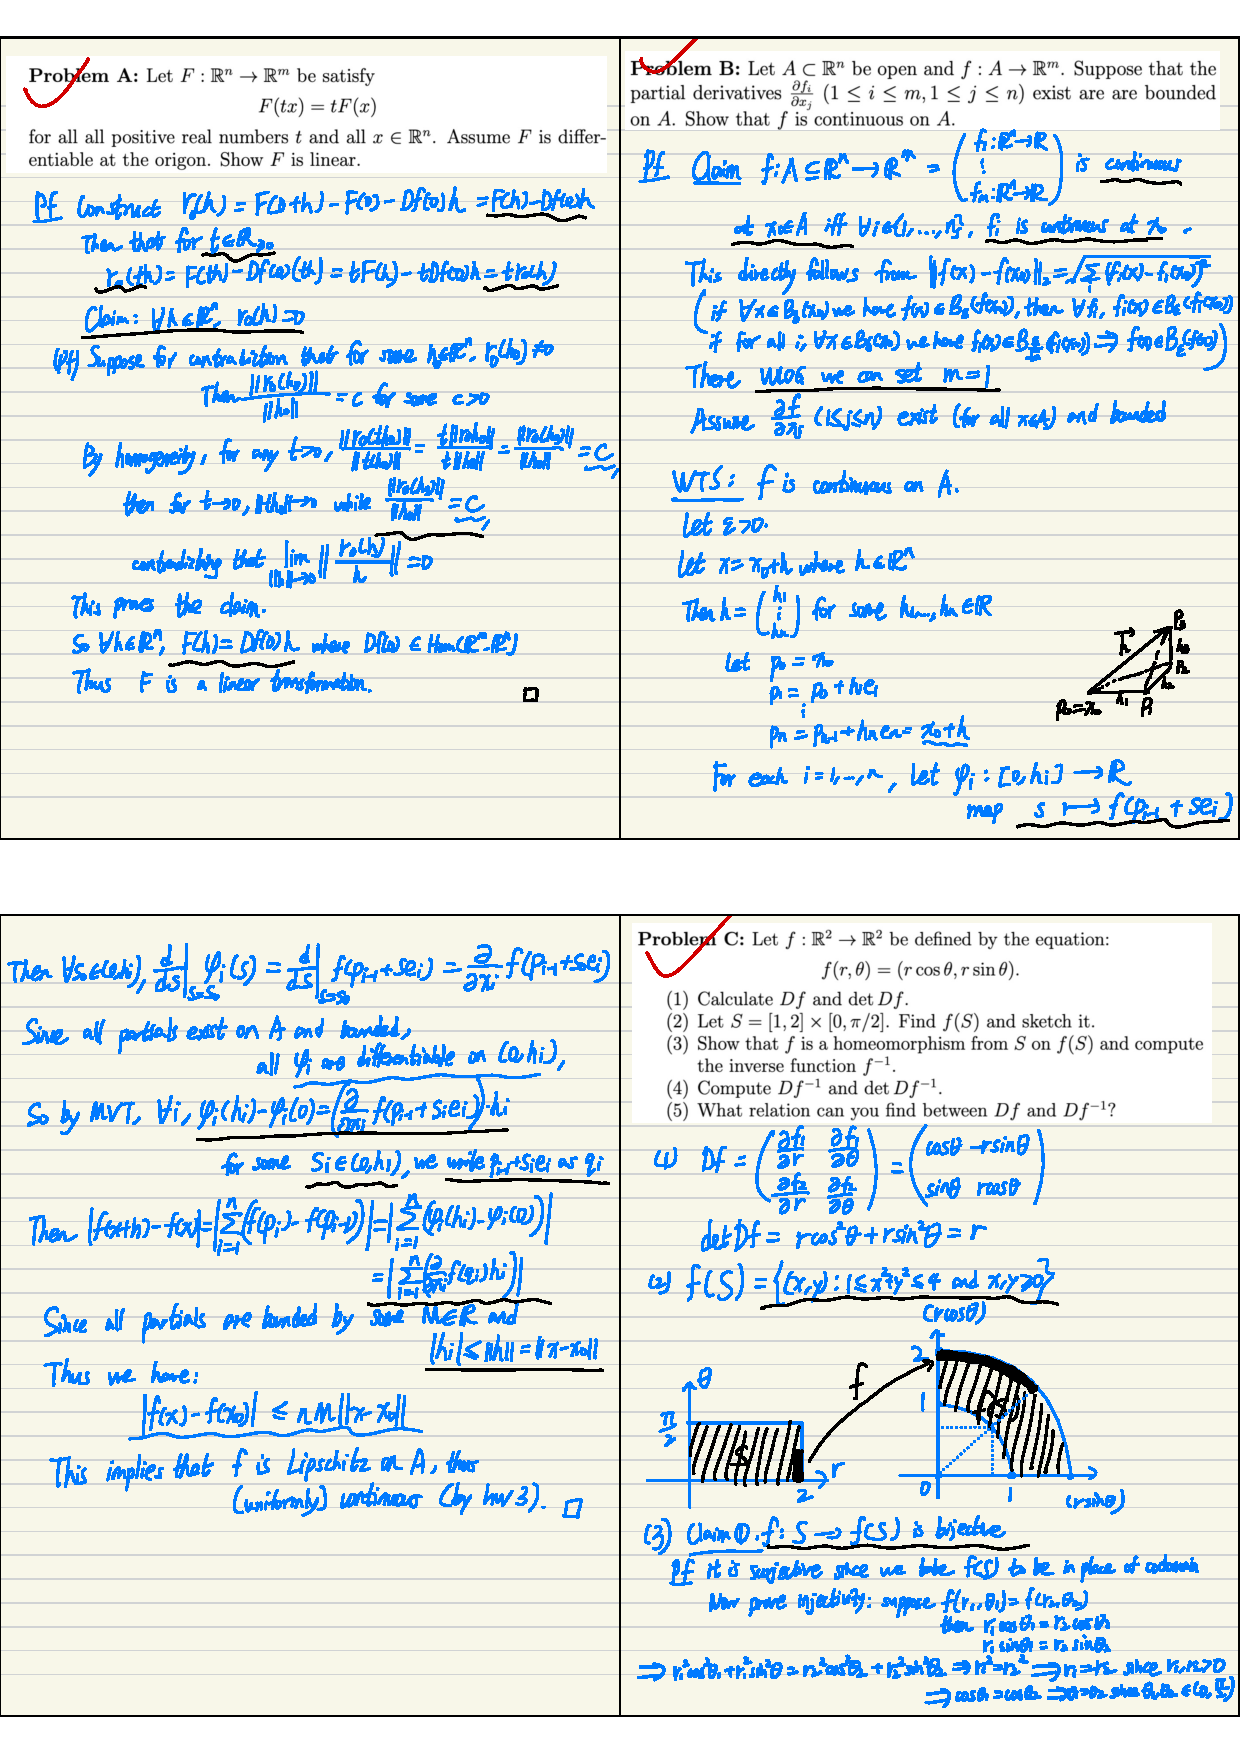
\includepdf[pages=-]{395-hw-04.pdf}



\chapter{on chain rule, prod rule and Taylor's Thm}

\section{applying chain rule to compute derivative}
Let $F : \mathbb{R}^3 \to \mathbb{R}^3$ be defined by
\[
F(x, y, z) = (\exp(x^2 + 2y^2), \sin(z^2 - y^2) \cdot (x^2 + 2z^2), (x^2 + y^2 + z^2)^9).
\]
Explain why $F$ is differentiable, and then prove why $DF(x, y, z)$ always has zero determinant. You may not actually compute any derivatives in your solution.

\section{diffeo 维度必须相同且 derivatives 互为 inverse matrix}
Suppose
\[
F : A \subset \mathbb{R}^n \to B \subset \mathbb{R}^m
\]
and
\[
G : B \subset \mathbb{R}^m \to A \subset \mathbb{R}^n
\]
are both differentiable and are inverses of each other (with $A$, $B$ open). Show that $n = m$ and that, for all pairs $a \in A$, $b \in B$ with $F(a) = b$,
\[
DG(b) = DF(a)^{-1}.
\]

\section{differentiable homeomorphism 未必是 diffeomorphism}
Give an example of a differentiable homeomorphism from $\mathbb{R}$ to itself whose inverse is not differentiable at every point. (For your example, you need to find only a single point where the inverse isn’t differentiable.)

\section{$f$ 在 $x_0$ 处 ctn $\implies$ 取多元极限可换序}
Suppose $F : \mathbb{R}^2 \to \mathbb{R}$ is continuous at the origin. Show
\[
\lim_{h \to 0} \lim_{k \to 0} F(h, k) = \lim_{k \to 0} \lim_{h \to 0} F(h, k),
\]
assuming all these limits exist. Give an example where $F$ is not continuous, both double limits exist, but the two double limits are not equal.

\textit{Just for fun (don’t hand in)}: Give an example where $F : \mathbb{R}^2 \to \mathbb{R}$ is continuous at the origin but $\lim_{h \to 0} \lim_{k \to 0} F(h, k)$ does not exist.

\textit{Just for fun (don’t hand in)}: Also note that for $a_{n,m} = 2^{n-m}$ it is not true that
\[
\lim_{n \to \infty} \lim_{m \to \infty} a_{n,m} = \lim_{m \to \infty} \lim_{n \to \infty} a_{n,m}.
\]

\section{number of terms in Taylor series}
If $F$ is a function of 4 variables, how many terms (in general) are in the degree 10 Taylor series of $F$? (Degree 10 means you use multi-indices $\alpha$ of degree at most 10.) You do not need to show your work; just give the final answer.

\section{open connected set 上 determinant 为 0 $\implies$ constant function}
Suppose that $F : A \subset \mathbb{R}^n \to \mathbb{R}^m$ is differentiable with $A$ open and connected and $Df(a) = 0$ for all $a \in A$. Show that $F$ is constant.

\section{multifunction product rule in 1d}
Let $f_1, f_2, \ldots, f_m : \mathbb{R} \to \mathbb{R}$ be $C^k$. Show that
\[
\frac{\partial^k}{\partial x^k}(f_1 \cdot f_2 \cdot \ldots \cdot f_m) = \sum_{|\alpha| = k} \frac{k!}{\alpha!} \partial^{\alpha_1} f_1 \cdot \ldots \cdot \partial^{\alpha_m} f_m.
\]


$$
\sum_{i=1}^m \frac{k!}{\beta_1 ! \cdots (\beta_i- 1)! \cdots \beta_m !}
$$
is it equal to 
$$
 \frac{(k+1)!}{\beta_1 !  \cdots \beta_m !}
$$


\section{proof: Taylor series is the best polynomial approximation}
Let $f : \mathbb{R}^n \to \mathbb{R}$ be in $C^{k+1}$. Show that the Taylor polynomial of degree $k$ centered at $x_0 \in \mathbb{R}^n$ is the best polynomial approximation of $f(x)$ near $x_0$ in the following sense: Suppose that $P(x)$ is a polynomial of degree $k$. Then
\[
P(x) - f(x) = o(|x - x_0|^k)
\]
if and only if $P$ is the Taylor polynomial of degree $k$ centered at $x_0$. (Recall that a quantity $Q$ is $o(|x - x_0|^k)$ if $\lim_{x \to x_0} \frac{Q}{|x - x_0|^k} = 0$.)


\noindent \textbf{5I: computation problem 1}
Let $f : \mathbb{R} \to \mathbb{R}$ be a differentiable function, and define $F : \mathbb{R}^2 \to \mathbb{R}$ by $F(x, y) = f(x^2 + y^2)$, so $F$ is differentiable.

\begin{enumerate}
    \item Prove that $x \frac{\partial F}{\partial y} = y \frac{\partial F}{\partial x}$.
    \item Suppose $f : \mathbb{R}^3 \to \mathbb{R}$, $g : \mathbb{R}^2 \to \mathbb{R}$, $h : \mathbb{R} \to \mathbb{R}$ are differentiable. Define $\phi : \mathbb{R}^3 \to \mathbb{R}^2$ via
    \[
    \phi(x, y, z) = (f(h(x), g(x, y), z), g(y, z)).
    \]
    Find a formula for the matrix of the derivative $D\phi(p) : \mathbb{R}^3 \to \mathbb{R}^2$ at an arbitrary point $p \in \mathbb{R}^3$ in terms of the partial derivatives of $f$, $g$, and $h$ at $p$.
    \item In (ii), compute $D\phi(1, 1, 1)$ when $f(x, y, z) = x^2 + yz$, $g(x, y) = y^3 + xy$, and $h(x) = e^x$. Do this in two ways: using your general formula in (ii) and also by explicitly computing $\phi$ in this case and directly computing the Jacobian matrix from this.
\end{enumerate}

\noindent \textbf{5J: computation problem 2}
Problem 2(a) on page 63 of the text.

\noindent \textbf{5K: computation problem 3}
Find the 3rd order Taylor series of $F(x, y) = e^{x + y^2}$ about the origin.

\section{Bonus: positive-definite matrix}
A real symmetric $n \times n$ matrix $A$ is called positive definite if $x^T A x > 0$ for all $x \in \mathbb{R}^n$.
\begin{enumerate}
    \item Show that a real symmetric matrix is positive definite if and only if it is invertible and, for all non-zero $x$, the angle between $Ax$ and $x$ is less than 90 degrees.
    \item Show that a real symmetric matrix is positive definite if and only if all its eigenvalues are positive.
    \item Let $A_d$ be the top left $d \times d$ minor of $A$. Show that if $A$ is positive definite, so is each $A_d$, $1 \leq d \leq n$.
    \item Prove that $A$ is positive definite if and only if $\det(A_d) > 0$ for all $1 \leq d \leq n$.
\end{enumerate}

You may use without proof that a real symmetric matrix has an orthonormal basis of eigenvectors. A hint for the last part is available on the office door, but as always, try it without first!



\includepdf[pages=-]{395-hw-05.pdf}






\chapter{on about IVT}

\section{MVT does not hold for $f: \bR \rightarrow \bR^n$}
Let $f : [a, b] \to \mathbb{R}^n$ be continuous on the closed interval $[a, b] \subset \mathbb{R}$ and differentiable on $(a, b)$.
\begin{enumerate}
    \item Show that there is a $c \in (a, b)$ such that
    \[
    |f(a) - f(b)| \leq |f'(c)| \cdot |a - b|.
    \]
    \item Give an example when $n = 2$ to show that it is possible the inequality is strict for all $c \in (a, b)$. (In particular, the Mean Value Theorem does not hold for $f$.)
\end{enumerate}

\noindent \textbf{6B}
Let $f : \mathbb{R}^2 \to \mathbb{R}^2$ be defined by the equation
\[
f(x, y) = (e^x \cos y, e^x \sin y).
\]
\begin{enumerate}
    \item Show that $f$ is one-to-one on the set $A = \{(x, y) : x \in \mathbb{R}, 0 < y < 2\pi\}$.
    \item What is $B = f(A)$?
    \item If $g$ is the inverse function of $f$ restricted to $A$, find $Dg(0, 1)$.
    \item What is $f(\mathbb{R}^2)$?
    \item Show that the Jacobian matrix of $f$ is nonsingular for any $(x, y) \in \mathbb{R}^2$. Thus every point of $\mathbb{R}^2$ has a neighborhood on which $f$ is one-to-one. Nonetheless, show that $f$ is not one-to-one on $\mathbb{R}^2$.
    \item Find an explicit formula for the inverse function $g$ of $f$ in the neighborhood of $(0, 1)$. Use this formula to check your answer in part (3).
\end{enumerate}


\section*{Problem C}
Suppose that $f : \mathbb{R} \to \mathbb{R}$ is continuous and locally invertible. Show that the image of $f$ is open, and that a global inverse for $f$ exists defined on the image.

\textit{Remark:} The analogue of Problem C is false in higher dimensions. You should pause to note what your solution uses that wouldn’t be available in higher dimensions.

\textit{Just for fun (don’t hand in):} Give an example of a continuous $f : \mathbb{R}^2 \to \mathbb{R}^2$ that is locally invertible but not injective.

\section*{Problem D}
Say that $f : \mathbb{R}^m \to \mathbb{R}$ is $C^\infty$, and there is a number $W > 0$ such that for all $x \in B_r(0)$ and all $\alpha$, we have
\[
|\partial^\alpha f(x)| \leq W |\alpha|.
\]
Show that
\[
\lim_{k \to \infty} \sum_{|\alpha| \leq k} \frac{\partial^\alpha f(0)}{\alpha!} x^\alpha = f(x)
\]
for $x \in B_r(0)$. Show also that the infinite series
\[
\sum_{\alpha} \frac{\partial^\alpha f(0)}{\alpha!} x^\alpha
\]
converges absolutely, so that without any ambiguity we can write
\[
f(x) = \sum_{\alpha} \frac{\partial^\alpha f(0)}{\alpha!} x^\alpha.
\]

\textit{Just for fun (don’t hand in):} $|\partial^\alpha f(x)| \leq W |\alpha|$ is not optimal. Can you phrase a natural assumption that is closer to optimal?

\section*{Problem E}
If $U \subset \mathbb{R}^n$ is open and $f : U \to \mathbb{R}$ is $C^1$ and has a local minimum at $x$, prove $Df(x) = 0$. (Points $x$ with $Df(x) = 0$ are called critical points.)

\section*{Problem F}
Let $f : A \to \mathbb{R}$ be a $C^2$ function, $A \subset \mathbb{R}^n$ open, and let $x \in A$. The Hessian $Hf(x)$ of $f$ at $x$ is the $n$-by-$n$ symmetric matrix with entry $(j, k)$ equal to $\partial e_i + e_k f(x)$.

A symmetric matrix $S$ is called positive definite if $x^T S x > 0$ for all $x \in \mathbb{R}^n$, $x \neq 0$, in which case we write $S > 0$. If the same condition holds with a non-strict inequality $x^T S x \geq 0$, we say $S$ is positive semi-definite and write $S \geq 0$. The negative of a positive (semi-)definite matrix is called negative (semi-)definite, and we similarly write $S < 0$ or $S \leq 0$.

Assume that $A$ is convex, and $Df(x_0) = 0$. Prove that:
\begin{enumerate}
    \item if $Hf(x) \geq 0$ for all $x \in A$, then $f(x) \geq f(x_0)$ for all $x \in A$.
    \item if $Hf(x) > 0$ for all $x \in A$, then $f(x) > f(x_0)$ for all $x \in A$.
    \item if $Hf(x) \leq 0$ for all $x \in A$, then $f(x) \leq f(x_0)$ for all $x \in A$.
    \item if $Hf(x) < 0$ for all $x \in A$, then $f(x) < f(x_0)$ for all $x \in A$.
    \item if $Hf(x_0) \not\geq 0$, then $f$ does not have a local minimum at $x_0$.
    \item if $Hf(x_0) \not\leq 0$, then $f$ does not have a local maximum at $x_0$.
\end{enumerate}

You only need to submit your proofs for parts (1) and (5); you don’t have to write up the rest.

\section*{Problem G}
Submit a write-up for Problem E on worksheet 5.

\section*{Bonus}
Let $M_n(\mathbb{R})$ denote the set of $n$-by-$n$ real matrices. It has a topology and metric by identifying with $\mathbb{R}^{n^2}$ using the entries of the metric.
\begin{enumerate}
    \item For any $A \in M_n(\mathbb{R})$, show that
    \[
    \lim_{K \to \infty} \sum_{k=0}^K \frac{A^k}{k!}
    \]
    exists. This limit is denoted
    \[
    \exp(X) = \sum_{k=0}^\infty \frac{A^k}{k!}.
    \]
    \item Compute $\exp$ of the following matrices:
    \[
    \begin{pmatrix} 0 & t \\ 0 & 0 \end{pmatrix}, \quad \begin{pmatrix} s & 0 \\ 0 & t \end{pmatrix}, \quad \begin{pmatrix} 0 & t \\ -t & 0 \end{pmatrix}.
    \]
    \item Show that $\exp(A + B) = \exp(A)\exp(B)$ when $A$ and $B$ commute.
    \item Prove that $\exp$ is differentiable at the origin and compute its derivative there.
    \item Is $\exp$ surjective?
    \item Is $\exp$ injective?
\end{enumerate}

\chapter{on IFT and Implicit Function Thm}

For hints, see office door. But try without the hints first. There are no IBL problems this week.

\section*{Problem A}
Suppose $A \subset \mathbb{R}^n$ is open and $f : A \to \mathbb{R}$ is differentiable at $x \in A$. Show that if $u$ is a unit vector in $\mathbb{R}^n$, then
\[
D_u f(x) \leq |Df(x)|,
\]
with equality if and only if $u = \frac{Df(x)}{|Df(x)|}$. Show that $D_u f(x) = 0$ if and only if $u$ is orthogonal to $Df(x)$.

\textbf{Remark}: Keeping in mind that for functions to $\mathbb{R}$, the Jacobian matrix is also called the gradient, this shows that the gradient is the direction of fastest change of the function. Similarly, the set of directions where the function does not change (to first order) is the perpendicular space to the gradient.

\section*{Problem B}
Suppose $U \subset \mathbb{R}^n$ is open and $f : U \to \mathbb{R}$ and $c : U \to \mathbb{R}$ are $C^1$. Set
\[
M = c^{-1}(0).
\]
Assume that $f$ restricted to $M$ has a local minimum at $p$, and that $Dc$ is surjective at $p$. Then prove that there exists a real number $\lambda$ such that
\[
Df(p) = \lambda Dc(p).
\]
(This means the gradients of $f$ and $c$ are parallel at $p$. The number $\lambda$ is called a \textit{Lagrange multiplier}.)

Hints: how that M can be parameterized, by implicit function theorem: M = {(x, g(x))} for a $g: \mathbb{R}^{n-1} \rightarrow \mathbb{R}$, show that kerDc = ImDg


\section*{Problem C}
In at most a few sentences, give a non-rigorous, intuitive explanation for Problem B.

\section*{Problem D}
Using Problem B, find the minimum of the function $f(x, y) = 3x + y$ on the unit circle centered at the origin in $\mathbb{R}^2$.

\section*{Problem E}
Formulate and prove a generalization of Problem B when $c$ maps to $\mathbb{R}^k$ rather than $\mathbb{R}$. (Whereas Problem B allows you to do certain optimization problems subject to one constraint, this lets you do some optimization problems subject to $k$ constraints. Your generalization will feature numbers $\lambda_1, \dots, \lambda_k$.)

\textbf{Remark}: You must do Problem B first and then Problem E. You may not reference E in your solution to B.

\section*{Problem F}
Prove that the set of positive definite matrices is open in the set of $n \times n$ symmetric matrices. (You may not use the bonus from HW5.)

\section*{Problem G}
Suppose $f : A \to \mathbb{R}$ is $C^2$, with $A \subset \mathbb{R}^n$ open. Suppose that $x_0$ is a critical point of $f$ and the Hessian of $f$ is positive definite at $x_0$. Prove that $x_0$ is a strict local minimum for $f$.

\section*{Problem H}
Let $A$ be an invertible $n \times n$ matrix. Let $C$ be its cofactor matrix, so $C_{ij} = (-1)^{i+j} \det(A_{ij})$, where $A_{ij}$ is the $(n-1) \times (n-1)$ matrix obtained by deleting row $i$ and column $j$ from $A$. Prove the following version of Cramer's rule:
\[
A^{-1} = \frac{1}{\det(A)} C^T,
\]
where $C^T$ denotes the transpose of $C$. (You may use the cofactor expansion of the determinant.)

\section*{Problem I}
Let $f, g : (a, b) \subset \mathbb{R} \to \mathbb{R}^n$ be differentiable. Show that
\[
(f \cdot g)'(t) = f'(t) \cdot g(t) + f(t) \cdot g'(t),
\]
where $\cdot$ denotes dot product and $f'(t)$ denotes $Df(t)$ (which in this case is a vector).

\section*{Bonus}
Suppose $f : A \to \mathbb{R}$ is $C^2$, with $A \subset \mathbb{R}^n$ open and convex. Show that the region above $f$, i.e.
\[
\{(x, y) \in A \times \mathbb{R} : y \geq f(x)\},
\]
is convex if and only if the Hessian of $f$ is positive semi-definite at each point of $A$.




\chapter{on about Implicit Function Thm}

\section*{Problem A}
Let \( f : \mathbb{R}^3 \to \mathbb{R}^2 \) be of class \( C^1 \) and such that \( f(1, 2, 3) = 0 \) and

\[
Df(1, 2, 3) =
\begin{bmatrix}
1 & 2 & 1 \\
1 & -1 & 1
\end{bmatrix}
.
\]

\begin{enumerate}
    \item Does the equation \( f(x, y, z) = 0 \) define implicitly a function of some of the variables in terms of the rest? If so, what variables can be expressed in terms of what others? Discuss all the possibilities.
    \item Suppose there is a function \( g : B \to \mathbb{R}^2 \) of class \( C^1 \) defined on an open set \( B \) of \( \mathbb{R} \) such that \( f(x, g(x)) = 0 \) for \( x \in B \) and \( g(1) = (2, 3) \). Compute \( Dg(1) \).
\end{enumerate}

\section*{Problem B}
Let \( f : \mathbb{R}^{k+n} \to \mathbb{R}^n \) be of class \( C^1 \) and suppose that \( f(a) = 0 \) and \( Df(a) \) has rank \( n \). Show that if \( c \in \mathbb{R}^n \) is sufficiently close to 0, then the equation \( f(x) = c \) has a solution.

\section*{Problem C}
Let \( B \) be a closed box, and \( f : B \to \mathbb{R} \) be a continuous function. Show that \( f \) is integrable.

\section*{Problem D}
Write up Problem D from the IBL worksheet (on countable sets).

\section*{Problem E}
Write up Problem G from the IBL worksheet (on countable sets).

\section*{Bonus}
A map \( T \) from a metric space \( (X, d) \) to itself is called a contraction mapping if there is a \( 0 \leq c < 1 \) such that
\[
d(T(x), T(y)) \leq c \cdot d(x, y)
\]
for all \( x, y \in X \).

\begin{enumerate}
    \item Show that every contraction mapping of a complete metric space has a unique fixed point.
    \item Suppose that \( f : \mathbb{R}^d \to \mathbb{R}^d \) is \( C^1 \), and \( Df(0) \) is invertible. Show that for \( \epsilon > 0 \) sufficiently small, if \( B \) is the closed ball of radius \( \epsilon \) around 0, then there is a \( \delta > 0 \) such that if \( |y| < \delta \)
    \[
    T(x) = Df(0)(x) + y - f(x)
    \]
    defines a contraction mapping from \( B \) to itself. (As part of this, you’ll have to show \( T(B) \subset B \).)
    \item Explain why this immediately implies that the image of \( f \) contains a neighborhood of \( f(0) \).
\end{enumerate}

\textit{Remark:} The point of this problem is to give the idea for a different proof of the Inverse Function Theorem. (This proof can be found in many textbooks, but don’t look!) Studying the proof from class will help you solve this question, and you can use the lemmas from class if you want to.






\chapter{on Riemann Integrability}

\section*{Problem A}
Let $f : X \to Y$ be a function between metric spaces. Show that the set of points at which $f$ is continuous is a countable intersection of open sets.

\section*{Problem B}
Suppose that $f(x) : [a, b] \to \mathbb{R}$ is non-decreasing and bounded. Show that $f$ is integrable.

\section*{Problem C}
Suppose that $f, g : [0, 1] \to \mathbb{R}$ are two integrable functions. Show that the function $F (x, y) : [0, 1]^2 \to \mathbb{R}$ given by $F (x, y) = f(x)g(y)$ is also integrable.

\section*{Problem D}
Let $f : [0, 1] \to \mathbb{R}$ be defined by setting $f(x) = 1/q$ if $x = p/q$ where $p$ and $q$ are positive integers with no common factor, and $f(x) = 0$ otherwise.
\begin{enumerate}
    \item Without using the characterization of Riemann integrable functions, show that $f$ is integrable.
    \item Show that $f$ is continuous except at a set of measure 0.
\end{enumerate}

\section*{Problem E}
Let $Q$ be a box in $\mathbb{R}^n$ and $f : Q \to \mathbb{R}$ be a bounded function. Show that if $f$ vanishes except on a closed set $B$ of measure zero, then $f$ is integrable.

\section*{Problem F}
Show that if $Q_1, Q_2, \dots$ is a countable collection of closed boxes covering some box $Q$, then $v(Q) \leq \sum v(Q_i)$.


\section*{Problem G}
Write out a proof of the following special case of the Implicit Function Theorem. Let $f : \mathbb{R}^2 \to \mathbb{R}$ be $C^1$, and suppose that $(x_0, y_0) \in \mathbb{R}^2$ is such that $f(x_0, y_0) = 0$ and $\frac{\partial f}{\partial y}(x_0, y_0) \neq 0$. Prove that there is an interval $I$ containing $x_0$ and a $C^1$ function $g : I \to \mathbb{R}$ such that $f(x, g(x)) = 0$ for all $x \in I$.

\section*{Problem H}
Write up Problem B from IBL worksheet 7, on the measure of an elementary set.

\section*{Problem I}
Write up Problem E from IBL worksheet 7, on countable unions of almost disjoint boxes.

\section*{Bonus}
For this question, you can use without proof that if $(a, b)$ is an open interval in $\mathbb{R}$, there is a smooth function which is positive on $(a, b)$ and zero elsewhere. (You can see explicit examples of such functions on the Wikipedia page on bump functions.)
\begin{enumerate}
    \item If $B$ is an open box in $\mathbb{R}^d$, show that there is a smooth function which is positive on $B$ and zero elsewhere.
    \item If $U$ is an open set in $\mathbb{R}^d$, show that there is a smooth function which is positive on $U$ and zero elsewhere.
    \item So in particular, nasty sets like the Cantor set can be level sets of smooth functions. Why doesn’t this contradict the Implicit Function Theorem? What more would you have to assume about $f$ to get that $f^{-1}(0)$ can’t be a nasty set like the Cantor set?
    \item Show that there exist two smooth functions $f, g : \mathbb{R}^2 \to \mathbb{R}$ such that the intersection of their graphs is the Cantor set in the $x$-axis.
\end{enumerate}




\chapter{on Riemann Integration}

\section*{Problem A: Integrability of the Maximum Function}
Let \( B \) be a box in \( \mathbb{R}^n \). Show that if \( f, g : B \rightarrow \mathbb{R} \) are both integrable, then so is the function \( M \) defined by
\[
M(x) = \max(f(x), g(x)).
\]

\section*{Problem B: Integrability of Absolute Value}
Let \( B \) be a box in \( \mathbb{R}^n \). Show that if \( f : B \rightarrow \mathbb{R} \) is integrable, then so is \( |f| \) and moreover
\[
\int_B f(x) \, dx \leq \int_B |f(x)| \, dx.
\]

\section*{Problem C: Dense Subset and Non-Integrability}
\begin{enumerate}
    \item Prove that there exists a dense subset \( S \subset [0, 1]^2 \) such that the intersection of \( S \) with any vertical line is at most one point, and the intersection of \( S \) with any horizontal line is at most one point.
    \item Let \( f(x, y) : [0, 1]^2 \rightarrow \mathbb{R} \) be the characteristic function of \( S \) (i.e., \( f(x, y) = 1 \) for \( (x, y) \in S \) and 0 otherwise). Show that \( f(x, \cdot) \) is an integrable function of \( y \) and \( f(\cdot, y) \) is an integrable function of \( x \), but \( f \) is not integrable on \( [0, 1]^2 \) as a function of two variables.
\end{enumerate}

\section*{Problem D: Equality of Mixed Partials}
Let \( A \) be an open subset of \( \mathbb{R}^2 \); and let \( f : A \rightarrow \mathbb{R} \) be \( C^2 \). Let \( Q \) be a box contained in \( A \).
\begin{enumerate}
    \item Use Fubini’s Theorem and the Fundamental Theorem of Calculus to show that
    \[
    \int_Q \frac{\partial^2}{\partial x \partial y} f(x, y) \, dx \, dy = \int_Q \frac{\partial^2}{\partial y \partial x} f(x, y) \, dy \, dx.
    \]
    \item Provide a new proof (other than the one given in class) of the equality of mixed partials \( \frac{\partial^2}{\partial x \partial y} f(x, y) = \frac{\partial^2}{\partial y \partial x} f(x, y) \).
\end{enumerate}

\section*{Problem E: Darboux and Riemann Integrability Equivalence}
Show that \( f : B \rightarrow \mathbb{R} \) is Darboux integrable if and only if \( f \) is Riemann integrable.

\section*{Problem F: Gradient and Hessian Transformations under Linear Map}
Given a function \( f : \mathbb{R}^n \rightarrow \mathbb{R} \) that is \( C^2 \) and an \( n \times n \) matrix \( A \), define a new function \( g(x) = f(Ax) \). Calculate \( Dg(0) \) in terms of \( Df(0) \) and \( A \). Also, calculate the Hessian of \( g \) at 0 in terms of the Hessian of \( f \) at 0.
\begin{proof}
    注意到:
    $$
    (H_f)_{\text{row i}} = D \frac{\partial f}{\partial x_i}
    $$
    这里我们用到 chain rule 的一个平凡 corollary:
    $$
    \frac{\partial u}{\partial x_i} = \sum_i \frac{\partial u}{\partial y_j} \frac{\partial y_j}{\partial x_i}
    $$
\end{proof}

\section*{Problem G: Degree Two Taylor Polynomial}
Given a function \( f : \mathbb{R}^n \rightarrow \mathbb{R} \) that is \( C^2 \), give a formula for the degree two Taylor polynomial of \( f \) at 0 in terms of the derivative and Hessian of \( f \) at 0.



\section*{Bonus: Discontinuity on Irrationals and Continuity on Rationals}
Show that there does not exist a function \( f : \mathbb{R} \rightarrow \mathbb{R} \) that is discontinuous on the irrationals and continuous on the rationals.






\chapter{on J-meas and Fubini's Thm}

\section*{Problem A: Taylor Polynomial and Linear Transformation}
Given a function \( f : \mathbb{R}^n \rightarrow \mathbb{R} \) that is \( C^2 \) and satisfies \( Df(0) = 0 \), show that there exists an invertible \( n \times n \) matrix such that the function \( g(x) = f(Ax) \) has a degree two Taylor polynomial at 0 of the form
\[
C + \sum a_i x_i^2
\]
where each \( a_i \) is a real number and \( C \) is a constant.

\section*{Problem B: Summation of Doubly Infinite Sequence}
Let \( a : \mathbb{N}^2 \rightarrow \mathbb{R}^+ \) be a non-negative doubly infinite sequence with \( a_{n,m} \) as the \((n,m)\) term. Show that
\[
\sum_{(n,m) \in \mathbb{N}^2} a_{n,m} = \sum_{n \in \mathbb{N}} \sum_{m \in \mathbb{N}} a_{n,m}.
\]

\section*{Problem C: Semiring Structure}
Check that \( \mathbb{R} = [0, \infty) \cup \{\infty\} \) is a semiring, with the expected definitions of addition and multiplication, and the definition \( 0 \cdot \infty = 0 \).

\section*{Problem D: Upper Semi-Continuity of Oscillation}
Let \( X \) be a metric space. A function \( f : X \rightarrow \mathbb{R} \) is upper semi-continuous at \( x_0 \) if
\[
\limsup_{x \rightarrow x_0} f(x) \leq f(x_0).
\]
Show that if \( g : \mathbb{R} \rightarrow \mathbb{R} \) is a bounded function, then \( x \mapsto \operatorname{osc} g(x) \) is upper semi-continuous.

\section*{Problem E: Compact Regions and Fubini's Theorem}
Consider a region \( S \subset \mathbb{R}^{n+1} \) that is simple if there exists a compact Jordan measurable set \( C \) and two bounded continuous functions \( \varphi, \psi : C \rightarrow \mathbb{R} \) such that
\[
S = \{ (x, t) \in \mathbb{R}^n \times \mathbb{R} : x \in C; \varphi(x) \leq t \leq \psi(x) \}.
\]
Here we assume that \( \phi \leq \psi \) on \( C \).

\begin{enumerate}
    \item Explain why \( S \) is compact.
    \item Show that \( \partial S = E_1 \cup E_2 \cup E_3 \) where
    \[
    E_1 = \{ (x, t) \in \mathbb{R}^n \times \mathbb{R} : x \in \partial C; \phi(x) \leq t \leq \psi(x) \},
    \]
    \[
    E_2 = \{ (x, t) \in \mathbb{R}^n \times \mathbb{R} : x \in C; t = \phi(x) \},
    \]
    \[
    E_3 = \{ (x, t) \in \mathbb{R}^n \times \mathbb{R} : x \in C; t = \psi(x) \}.
    \]
    \item Show that \( E_1, E_2, E_3 \) all have Lebesgue measure 0.
    \item Conclude that \( S \) is Jordan measurable.
    \item Prove Fubini's theorem for simple regions: Let \( f : S \to \mathbb{R} \) be a continuous function. Then \( f \) is integrable over \( S \), and
    \[
    \int_S f = \int_C \left( \int_{t = \phi(x)}^{t = \psi(x)} f(x, t) \, dt \right) dx.
    \]
\end{enumerate}


\section*{Problem F: Integrability Over Open Sets}
Let \( A \) be an open subset of \( \mathbb{R}^n \), and let \( f : A \rightarrow \mathbb{R} \) be continuous. Prove that \( \int_A f \) exists in the extended sense if and only if \( \int_{U_N} |f| \) is bounded, where \( U_1 \subset U_2 \subset \dots \) is a sequence of open sets whose union is \( A \).

\section*{Problem G: Integrability of Functions over Specified Sets}
For each function \( f \) and set \( A \), determine whether \( f \) is integrable over \( A \) and calculate \( \int_A f \).

\section*{Problem H: Jordan Measurability and Measure Calculation}
Show that the set 
\[
\{ (x_1, \dots, x_n) \in [0, 1]^n : \sum x_i \leq 1 \}
\]
is Jordan measurable and compute its measure.

\section*{Bonus: Nowhere Dense Subset with Positive Measure}
Construct a closed, nowhere dense subset of \([0,1]\) that does not have measure 0.








\chapter{applications of COV}

\section*{12A: Integration on Bounded Sets}
Let \( S \) be a bounded set in \( \mathbb{R}^n \), and let \( f : S \rightarrow \mathbb{R} \) be a bounded continuous function; let \( A = \text{Int}(S) \) be the interior of \( S \). Suppose that \( f \) is integrable on \( S \).

1. Show that \( f \) is integrable on \( A \) and that
   \[
   \int_A f = \int_S f.
   \]

2. Deduce that if \( S \) is Jordan measurable, then \( A \) is Jordan measurable as well and \( m(A) = m(S) \).

Warning: \( A \) is always Lebesgue measurable, since \( A \) is open and open sets are Lebesgue measurable. However, for example, when \( S = [0, 1] \setminus \mathbb{Q} \), it’s possible to have \( S \) Lebesgue measurable but for \( A \) and \( S \) to have different Lebesgue measures. Such examples must have \( S \) not Jordan measurable.

\begin{proof}
    $f$ Riemann integrable on $S$, so $m(D_f) = 0$ and $m(\{x_0 \in \partial S | \lim_{x \rightarrow x_0} f(x)  \not = 0  \}) = 0$.\\
    My question: Since $f$ is ctn on $S$, does it mean that for all $x_0 \in S - \partial S $, $\lim_{x \rightarrow x_0} f(x) = f(x_0)$? 
\end{proof}




\section*{12B: Volume of Balls in \( \mathbb{R}^n \)}
Let \( B^n_a(x) \) denote the ball in \( \mathbb{R}^n \) centered at \( x \) and radius \( a \).

1. Show that
   \[
   \text{vol}(B^n_a(x)) = \Gamma_n a^n
   \]
   where \( \Gamma_n = \text{vol}(B^n_1(0)) \).

2. What is \( \Gamma_1 \) and \( \Gamma_2 \)?

3. Compute \( \Gamma_n \) in terms of \( \Gamma_{n-2} \), and deduce a formula for \( \Gamma_n \) for any \( n \).

Just for fun, don’t hand it in: As the dimension gets large, what happens to the volume of the unit ball divided by the volume of \( [-1, 1]^n \) (the smallest box containing the unit ball)? If you pick a point at random in the box, is it likely to be in the ball?

\section*{Problem C: Volume of a Cone Over an Open Set}
Let \( A \) be an open Jordan measurable set in \( \mathbb{R}^{n-1} \). Given a point \( p \in \mathbb{R}^n \) with \( p_n > 0 \), let \( S \) be the subset of \( \mathbb{R}^n \) defined by
\[
S = \{ (1 - t)a + tp : a \in A \times \{0\}, 0 < t < 1 \}.
\]
(S is the union of all open line segments in \( \mathbb{R}^n \) joining \( p \) to points of \( A \times \{0\} \). You might think of it as a cone over \( A \).)

1. Define a diffeomorphism \( g \) of \( A \times (0, 1) \) with \( S \).

2. Find the volume of \( S \) in terms of the area of \( A \).

\section*{12D: Volume of Ellipsoid}
Compute the volume inside the ellipsoid
\[
\frac{(x - u)^2}{a^2} + \frac{(y - v)^2}{b^2} + \frac{(z - w)^2}{c^2} = 1
\]
where \( a, b, c > 0 \) and \( u, v, w \in \mathbb{R} \).

\section*{12E: Volume of a Solid Bounded by a Surface and Plane}
Compute the volume of the solid in \( \mathbb{R}^3 \) bounded below by the surface \( z = x^2 + 2y^2 \) and above by the plane \( z = 2x + 6y + 1 \).

\section*{12F: Gaussian Integral}
Evaluate
\[
\int_{-\infty}^{\infty} e^{-x^2} \, dx.
\]

\section*{12G: Integrability of \( |x|^e \) Over the Unit Ball and Its Complement}
For which exponents \( e \in \mathbb{R} \) is \( f(x) = |x|^e \) integrable over the unit ball in \( \mathbb{R}^n \)? For which exponents is it integrable over the complement of the closed unit ball?

\section*{Bonus: Proving a Case of Sard’s Theorem}
The purpose of this bonus is to prove the easiest case of Sard’s Theorem, a central tool in the study of manifolds.

1. If \( f : \mathbb{R} \rightarrow \mathbb{R} \) is continuous and \( I \) is a compact interval, then \( f(I) \) is a compact interval. (You don’t need to prove this; it follows easily from the fact that a continuous image of a compact set is compact and a continuous image of a connected set is connected.) Show that if \( f \) is differentiable with \( |f'| \leq \delta \) on \( I \), then
   \[
   |f(I)| \leq \delta |I|,
   \]
   where \( |I| \) denotes the length of an interval \( I \).

2. Suppose \( f : \mathbb{R} \rightarrow \mathbb{R} \) is \( C^1 \). Show that
   \[
   f(\{x \in \mathbb{R} : f'(x) = 0\})
   \]
   has measure zero. You should do this by first showing that for each \( n \),
   \[
   f(\{x \in [-n, n] : f'(x) = 0\})
   \]
   has measure zero, using that \( f' \) is continuous and hence uniformly continuous on \( [-n, n] \).





\chapter{on smooth functions}

\section{Matrix decomposition}
Write the matrix 
\[
\begin{pmatrix}
0 & 1 \\
1 & 0
\end{pmatrix}
\]
as a product of \(2 \times 2\) matrices that are primitive diffeomorphisms. You need only give the final answer.
\begin{solution}
    This is just the matrix of swapping row 1 and row 2.\\ Apply procedure at page 157.
\end{solution}


\section{POU sDominated by open cover}
Explicitly give a partition of unity of \( \mathbb{R} \) dominated by the cover by all open intervals of length 7.
\begin{solution}
    just the bump function supported on $[-3,4, 3.4]$, for each $n$ translated by $n$ (onto left if odd, onto right if even).
\end{solution}

\section{Smoothness of $e^{-1/x}$}
Show that the function \( f : \mathbb{R} \to \mathbb{R} \) defined by:
\[
f(x) =
\begin{cases} 
e^{-1/x} & \text{if } x > 0, \\
0 & \text{otherwise}
\end{cases}
\]
is \( C^\infty \). (For hints, see page 143 of the text.)
\begin{proof}
It is smooth on $x<0$, $X>0$ since it is composed of fundamental smooth functions.\\
So it remains to show that the function is infinite-times differentiable at $x = 0$.
\end{proof}

\section*{13D}
If \( f : \mathbb{R}^n \to \mathbb{R}^m \) is smooth and \( n < m \), show that the image cannot contain an open set.

\section*{Problem E: Super-Primitive Diffeomorphisms}
Define a diffeomorphism to be super-primitive if it preserves all but one coordinate. Show that the theorem proved in class on locally factoring diffeomorphisms remains true if one replaces primitive with super-primitive.
\begin{proof}

    
\end{proof}


\section*{13F}
Show that there is no injective smooth function \( f : \mathbb{R}^2 \to \mathbb{R} \).

\section*{Problem G: Smooth Functions on Arbitrary Subsets}(Mun Page 144)
For an arbitrary subset \( S \subset \mathbb{R} \) and a function \( f : S \to \mathbb{R} \), we say that \( f \) is smooth at \( x \in S \) if there is an open set \( U_x \) containing \( x \) and a smooth function \( f_x : U_x \to \mathbb{R} \) such that \( f \) and \( f_x \) agree on \( U_x \cap S \). Show that if \( f \) is smooth at every point of \( S \), then there is an open set \( V \) containing \( S \) and a smooth function \( g : V \to \mathbb{R} \) that agrees with \( f \) on \( S \).

\section*{Problem H: Rank of a Matrix}
Let \( A \) be a matrix. Show that the rank of \( A \) is the maximum value of \( k \) such that a \( k \times k \) minor of \( A \) has a non-zero determinant. (A \( k \times k \) minor is a matrix obtained by deleting all but \( k \) rows and all but \( k \) columns.)

\section*{Bonus: Composition of Primitive Diffeomorphisms}
Prove or disprove: Every diffeomorphism between connected open subsets of \( \mathbb{R}^n \) (where \( n \geq 2 \)) can be (globally) expressed as a composition of primitive diffeomorphisms between open subsets of \( \mathbb{R}^n \).





\chapter{HW 14}

\section{seq of smooth functions that sum to be disctn}
Construct a sequence of smooth functions $\psi_i : \mathbb{R} \to \mathbb{R}$ with disjoint supports such that the function $\lambda : \mathbb{R} \to \mathbb{R}$ defined by
\[
\lambda(x) = \sum_{i=1}^\infty \psi_i(x)
\]
is not continuous.

\textbf{Hint:} Try letting $\psi_i$ be a bump function supported on $[1/2^{2i+2}, 1/2^{2i+1}]$.

\textbf{Remark:} This problem illustrates why, in the definition of a partition of unity, we require that each point has a neighborhood that intersects only finitely many supports, rather than just saying that for each $x$ only finitely many of the functions are non-zero at $x$.

\section{Proving COV for linear diffeos and ctns functions with cpt supp}
Prove the Change of Variable Theorem for linear diffeomorphisms and continuous functions with compact support. You can use results proved in class up to and including the result that every linear diffeomorphism is a composition of primitive linear diffeomorphisms. You cannot use results proved after that.

\textbf{Remark:} This will not take very long. Because the functions have compact support, the integrals can be interpreted as ordinary integrals, and one can proceed directly to the punchline with Fubini. The purpose of this problem is to help you study the “core” of the proof of Change of Variables without getting lost in the technical details.

\section{rank function is semi-continuous on $M_{n,m}$}
Let $M_{n,m}$ be the space of $n \times m$ matrices. Show that the rank function is lower semi-continuous on $M_{n,m}$. Provide an example to show it need not be continuous.

\textbf{Hint:} To prove lower semi-continuity, you need to show every matrix $A$ has a neighborhood whose rank is at least as big as the rank of $A$. You can do this quickly using the problem from the last homework on rank. For the example, consider small multiples of the identity.










\chapter{Homework Set 15}

\section{Nonexistence of injective smooth function from higher dim to lower dim}
Prove that there does not exist an injective smooth function \( f : \mathbb{R}^n \to \mathbb{R}^m \) when \( n > m \).

\section{Convolution of continuous functions}
Let \( f, g : \mathbb{R}^n \to \mathbb{R} \) be continuous functions that are zero outside a compact set. Define their convolution as
\[
(f \ast g)(x) = \int_{\mathbb{R}^n} f(x-y)g(y) \, dy.
\]
Show the following:
1. \(\int_{\mathbb{R}^n} f \ast g = \left( \int_{\mathbb{R}^n} f \right) \left( \int_{\mathbb{R}^n} g \right)\),
2. Convolution is commutative and associative.

\section{Optimization of a quadratic function on a disk}
Find the maximum and minimum values of \( f(x, y) = 4x^2 + 10y^2 \) on the disk \( x^2 + y^2 \leq 4 \).

\section{expressing tensors}
Determine which of the following functions on \( \mathbb{R}^4 \) are tensors, and express those that are as elementary tensors:
\[
f(x, y) = 3x_1y_2 + 5x_2x_3, \quad g(x, y) = x_1y_2 + x_2y_4 + 1, \quad h(x, y) = x_1y_1 - 7x_2y_3.
\]

\section{$\cL^k(V)$ is a vector space}
Let $V$ be a vector space, and $\cL^k(V)$ be the space of all k-tensors on $V$. Prove: $\cL^k(V)$ is a vector space.

\section*{15F: compute the sign of a permutation}
Let \( \sigma \in S_k \) be the permutation described by
\[
1 \to 2 \to 3 \to \cdots \to k \to 1.
\]
Compute the sign of \( \sigma \).

\section{dual of alternating \(k\)-tensor is also alternating \(k\)-tensor}
Let \( T : V \to W \) be a linear transformation. If \( f \in A^k(W) \), show that \( T^\ast(f) \in A^k(V) \).

\section{Reproducing Theorem 27.7}
Prove Theorem 27.7: Let $\psi_I$ be an elementary alternating tensor on $\bR^n$ correspoding to the usal basis for $\bR^n$, where $I = (i_1, \cdots, i_k)$. \\
Given vectors $x_1, \cdots, x_k$ of $\bR^n$, let $X$ be the matrix $X = [x_1, \cdots, x_k]$. Then we have:
$$
\psi_I (x_1, \cdots, x_k) = \det X_I
$$

\section{Bonus: Analytic functions and series convergence}
Consider the function \( f : (0, 1) \to \mathbb{R} \) defined by
\[
f(p) = \sum_{n=1}^\infty a_n p^{k_n}(1-p)^{n-k}.
\]
where \( a_n \in \{0, 1\} \) and \( 0 \leq k_n \leq n \). Show the following:
1. \( f \) is real analytic.
2. For a power series \( f(x) = \sum_{n=0}^\infty c_n(x-x_0)^n \), define the radius of convergence as
\[
R = \frac{1}{\limsup_{n \to \infty} |c_n|^{1/n}},
\]
and show that the series converges uniformly and absolutely for \( x \in (x_0 - R, x_0 + R) \) and diverges for \( x \not\in [x_0 - R, x_0 + R] \).
3. If the series converges on \( (x_0-r, x_0+r) \) for some \( r > 0 \), then for any \( 0 < \rho < r \), there exists a constant \( C \) such that \( |c_n| \leq C \rho^n \).
4. Conclude that \( f'(x_0) \) exists and is equal to \( c_1 \).

\textbf{Remark:} The final part demonstrates that real analytic functions are smooth. The proof involves showing that \( f \) is \( C^\infty \) by defining \( g(x) = \sum_{n=1}^\infty n c_n (x-x_0)^{n-1} \), and leveraging results about uniform convergence of derivatives.



\end{document}
